\documentclass[5pt]{report}
\usepackage[utf8]{inputenc}
\usepackage[spanish]{babel}
\usepackage{amsmath}
\usepackage{amsfonts}
\usepackage{amssymb}
\usepackage{graphicx}
\usepackage{ragged2e}
\usepackage{lettrine}
\usepackage{float}
\usepackage{adjustbox}
\usepackage{geometry}
\usepackage{afterpage}
\usepackage{steinmetz}
\usepackage{multicol}
\usepackage{lipsum}
\usepackage{booktabs}

\makeatletter
\def\hlinewd#1{%
\noalign{\ifnum0=`}\fi\hrule \@height #1 %
\futurelet\reserved@a\@xhline}
\makeatother

\geometry{
	a4paper,
	total={170mm,257mm},
	left=20mm,
	top=20mm,
}


\begin{document}
 \begin{center}
 		\begin{adjustbox}{width=\textwidth}
 		 	\centering
 		 	\begin{tabular} {| c | c | c | c |}
 		 		
 		 		\multicolumn{4}{c}{\raisebox{-\totalheight}{
\includegraphics[width=0.1\textwidth, height=10mm]{Logo_UTN-FRBA}} } \\
 		 		\multicolumn{4}{c}{ }\\
 		 		\hline
 		 		\multicolumn{4}{|c|}{\textbf{\scriptsize{UNIVERSIDAD TECNOLÓGICA NACIONAL}}}\\
 		 		\multicolumn{4}{|c|}{\scriptsize{FACULTAD REGIONAL Buenos Aires}}\\
 		 		\multicolumn{4}{|c|}{\scriptsize{Departamento de Electrónica}}\\
 		 		\hlinewd{2pt}
 		 		\multicolumn{4}{|c|}{\tiny{Cátedra: Técnicas Digitales II - Plan 1995 (Adecuado)}}\\
 		 		\hlinewd{2pt}
 		 		\multicolumn{4}{|c|}{ANTEPROYECTO}\\
 		 		\hline
 		 		\multicolumn{4}{c}{ }\\
 		 		\hline
 		 		\scriptsize{Grupo N$^\circ$ : 2} & \hfill & \scriptsize{Año y División: }& \scriptsize{2018 - R4001 }\\
 		 		\hline
 		 		\multicolumn{2}{|l|}{\scriptsize{Integrantes:}} & \multicolumn{2}{|l|}{\scriptsize{1 .- BANDA BORJA, Christian }}\\
 		 		\multicolumn{2}{|l|}{\scriptsize{}} & \multicolumn{2}{|l|}{\scriptsize{2 .- HIGA, Sebastián Ariel }}\\
 		 		\multicolumn{2}{|l|}{\scriptsize{}} & \multicolumn{2}{|l|}{\scriptsize{3 .- MUENA, Guillermo Ariel }}\\
 		 		\hline
		 		 \scriptsize{} & \scriptsize{\hfill} &\scriptsize{Fecha:}   &\scriptsize{23-04-2018} \\ 
		 		 \hline
		 		 \scriptsize{Título del Proyecto:} & \multicolumn{3}{|l|}{  \scriptsize{Monitor de señales vitales}} \\
		 		 \hline 
		 		 \multicolumn {4}{c}{  }\\
		 		 \multicolumn{4}{l}{\scriptsize{\textbf{Descripción}}}\\
		 		 \hline 
		 		 \multicolumn{4}{|c|}{  }\\
		 		 \multicolumn {4}{|l|}{ \parbox{0.5\textwidth}{\scriptsize{En este proyecto se desarrollará un monitor de señales vitales de uso hogareño. Se pretende que una persona sin conocimientos de medicina y/o conocimientos técnicos pueda manipularlo sin mayores complicaciones.Desde el punto de vista concreto de esta materia se hará una central de mediciones manejada por el LPC 1769 que cuente con los siguientes sensores: un medidor de temperatura corporal (termómetro), una balanza, y un medidor de tensión arterial. Tanto el termómetro como la balanza estarán directamente conectados a la placa controladora donde se encuentre alojado el LPC, mientras que el tensiómetro, que se realizará como proyecto para la cátedra de Medidas Electrónicas 1, será una entidad externa que se comunicará inalámbricamente con el LPC (se ha hablado con los profesores y queda la opción de hacerlo a través de tecnología Bluethooth o a través de tecnología Wi-Fi. Los integrantes de este grupo se reservan el derecho de elegirlo con posterioridad a la redacción de este anteproyecto, hasta establecer tanto el presupuesto y como la disponibilidad de hardware en el mercado local).  }}}\\
 		 		\hline
 		 	\end{tabular}
	 	\end{adjustbox}
	 	\newpage
	 		\begin{adjustbox}{width=\textwidth}
	 			\centering
	 			\begin{tabular} {| c | c | c | c |}
	 				\multicolumn{4}{c}{  }\\
	 				\hline
	 				\multicolumn{4}{|c|}{  }\\
	 				\multicolumn {4}{|l|}{ \parbox{0.5\textwidth}{\scriptsize{En cuanto a la interfaz del sistema, se utilizará un TFT color de tamaño mediano (con una GUI adecuada)que permita la fácil manipulación y que se montará directamente por encima de la placa que contenga el LPC. \newline También como parte de la interfaz de usuario se adicionará un método de conexión con PC y la respectiva GUI. \newline Como método de almacenaje de datos se utilizarán dos modos. Uno interno utilizando una memoria del tipo I2C, y un método de exportación, que permita migrar todos los datos almacenados a una memoria externa SD para su fácil transporte. \newline Cómo idea general se pretende que haya dos métodos de entradas de datos al sistema: mediciones directas a través de los sensores adicionados y un método de entrada manual de dichos datos. } }}\\
	 				\multicolumn{4}{|c|}{  }\\
	 				\hline
					 \multicolumn {4}{c}{  }\\
					 \multicolumn{4}{l}{\scriptsize{\textbf{Especificación Técnica}}}\\
					 \hline 
					 \multicolumn {4}{|c|}{  }\\
					 \multicolumn {4}{|l|}{ \parbox{0.5\textwidth}{\scriptsize{Específicamente se usarán los siguientes sensores: una termocupla para el cálculo de la temperatura corporal, cuyos valores de lectura sean procesados directamente por el ADC del microcontrolador; y un sensor de presión resistivo para implementar la balanza, también directamente conectado al ADC del micro. \newline Para interfaz de usuario se usará: una pantalla TFT táctil y una GUI para la misma; y una interfaz en PC (desarrollada en QTcreator probablemente, pero esa decisión se dejará para más adelante) comunicada por serie con el microcontrolador. \newline Como método de almacenamiento se usará una memoria controlada por I2C y la opción de migrar los datos a una SD. \newline Para el tensiómetro no se darán muchos detalles técnicos ya que su desarrollo responde a otra cátedra, y uno de los requisitos obligatorios para la presentación del mismo es no solo una documentación técnica detallada, sino también un manual completo de utilización y calibración. Sólo se dirá que se utilizará un módulo de comunicación wireless a definir en las próximas semanas y que al momento de entregar el informe final del proyecto se adjuntará toda la documentación pertinente.  } }}\\
					 \multicolumn {4}{|c|}{  }\\
					 \hline
	 			\end{tabular}
	 		\end{adjustbox}
 	\end{center}
	 	\newpage 
	 	\Large{\textbf{Diagrama en bloques}}
	 	\hrule
	 	\begin{figure} [H]
		\centering
		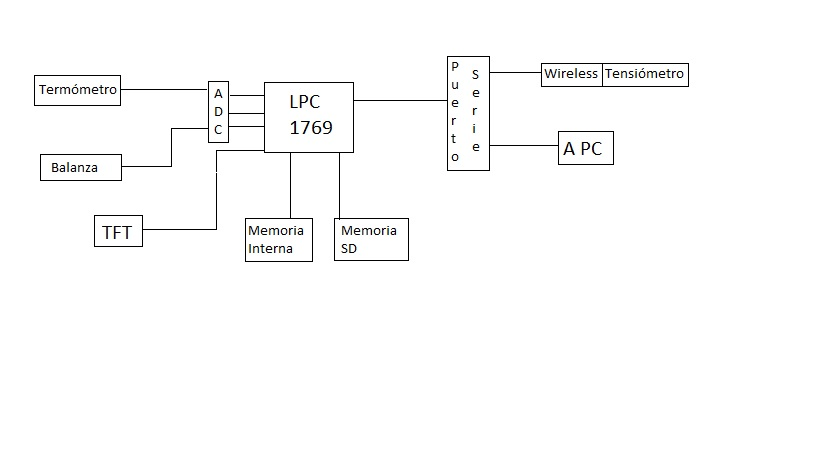
\includegraphics[width=1.2\linewidth]{guiie}
		\label{fig:guiie}
		\end{figure}
		
	 	\begin{adjustbox}{width=\textwidth}
	 		\centering
	 		\begin{tabular} {| c | c | c | c |}
	 			\multicolumn{4}{c}{  }\\
		 		\hline
	 			\multicolumn {4}{|c|}{  }\\

	 			\multicolumn {4}{|c|}{  }\\
	 			\multicolumn {4}{|c|}{.....................................................................................}\\	 	\multicolumn{4}{|c|}{\large{\textbf{Firma y aclaración del representante}}}\\
	 			\multicolumn {4}{|c|}{  }\\
	 			\hline
	 		\end{tabular}
	 	\end{adjustbox}

\end{document}
